\documentclass[12pt]{article}
\usepackage[a4paper,margin=.5in]{geometry}
\usepackage{graphicx}
\usepackage{booktabs}
\usepackage{listings}
\usepackage{color}

\definecolor{dkgreen}{rgb}{0,0.6,0}
\definecolor{gray}{rgb}{0.5,0.5,0.5}
\definecolor{mauve}{rgb}{0.58,0,0.82}

\lstset{frame=tb,
  language=Python,
  aboveskip=3mm,
  belowskip=3mm,
  showstringspaces=false,
  columns=flexible,
  basicstyle={\small\ttfamily},
  numbers=none,
  numberstyle=\tiny\color{gray},
  keywordstyle=\color{blue},
  commentstyle=\color{dkgreen},
  stringstyle=\color{mauve},
  breaklines=true,
  breakatwhitespace=true,
  tabsize=3
}
%\usepackage{subfig}
\usepackage{subcaption}
\usepackage{hyperref}
\hypersetup{
    colorlinks=true,
    linkcolor=blue,
    filecolor=magenta,      
    urlcolor=cyan,
    pdftitle={Overleaf Example},
    pdfpagemode=FullScreen,
    }
\newcommand*{\figuretitle}[1]{%
    {\centering%   <--------  will only affect the title because of the grouping (by the
    \textbf{#1}%              braces before \centering and behind \medskip). If you remove
    \par\medskip}%            these braces the whole body of a {figure} env will be centered.
}
\title{Final Project Progress Report}

\author{Tylman Michael\\CSE 546 Machine Learning}
\date{4/17/2023}
%moderncv theme
\usepackage[utf8]{inputenc} 
\begin{document}
\maketitle{}
\section{Initial Plan}
To begin on this project, I sat down with the requirements and wrote down what I had planned to do for each of them, 
given my knowledge about the problem and what methods were likely to be the best options for each. I will discuss them 
in the order I decided them, not necessarily the order listed for the assignment. For phase one, I wanted to handle 
which classifiers I was planning on using, which data normalization techniques works best for each, and what are the 
dimensionality reduction needs for each classifier

\subsection{4 Different Classifiers}
I wanted to include 2 classifiers that I felt like had the highest chance of success, and 2 classifiers that I felt like 
are foundational for Machine Learning which are important for me to get more experience in. As such for the two I felt like would do well, 
I chose to go with a Multi Layer Perceptron Neural Network (MLPNet for short), and a kernel SVM. 

I chose the MLPNet because I feel like since our 
dataset is described by a feature set created by a CNN, then an MLPNet is the most logical solution since that is likely 
the most similar achitecture to what the CNN was using to generate the optimal kernel weights for feature generation. I chose the kernel SVM because I'm aware that in the history of Machine Learning, before neural networks and deep learning 
took over, these models were usually the go-to option and the best performing.

For the two "Foundational" classifiers that I felt I need more experience with, I went with the Gaussian Naive Bayes 
classifier (GNB), and the Random Forest classifier (RF). I chose the GNB because I think it will provide a good insight 
on the training data, and give a good baseline from which we can draw conclusions to influence future decisions given it's 
extreme mathematical grounding. I chose the RF because I'm aware that it is a very popular technique that is utilized 
often in bioinformatics. In fact, my start in data science was working on improving the classification of central 
nervous system cancers which was started by a paper which used a random forest classifier on the methylation array data.


\subsection{Data Normalization} 
For the 2 data normalizations required, I picked the standard scaler and the minmax scaler. I chose the standard scaler
because it assumes a normal distribution, which the GNB classifier could use well, and everything's nicer when the 
standard normal distribution is assumed. Secondly, I chose the minmax scaler because I wanted to utilize the SVM and 
MLPNet classifiers, both of which historically work best and train fastest when the data is scaled between 0 and 1.

\subsection{PCA}
I originally planned to be more scientific about my choice of PCA components. I had planned to plot the total 
variance captured, and find both the elbow point of variance, and the 95 percent variance mark. I successfully 
did both of these experiments as shown in \ref{figure1}, but I quickly discoverd that I could instead pass the 
desired amount of variance directly to sklearns PCA function. 

Once I discovered this, I realized I could include this within a gridsearch so I could see if different classifiers 
have different dimensionality reduction needs. So, I combined seaching for optimal PCA variance and optimal 
normalization into the same first experiment, which I will talk more on later. 

However, one important takeaway from this is that I can keep 95\% of the total variance of the data while cutting my 
dimensionality by more than half. This is huge for rapid experimentation, and something I will absolutely abuse.

\begin{figure}
    \begin{subfigure}{.5\textwidth}
        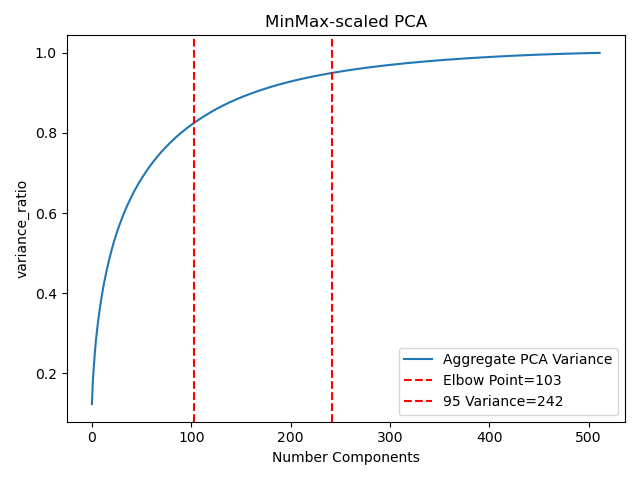
\includegraphics[width=.95\textwidth]{../../results_Experiment1/MinMax_PCA_choice.png}
        \caption{MinMax PCA Variance}
        \end{subfigure}%
      \begin{subfigure}{.5\textwidth}
        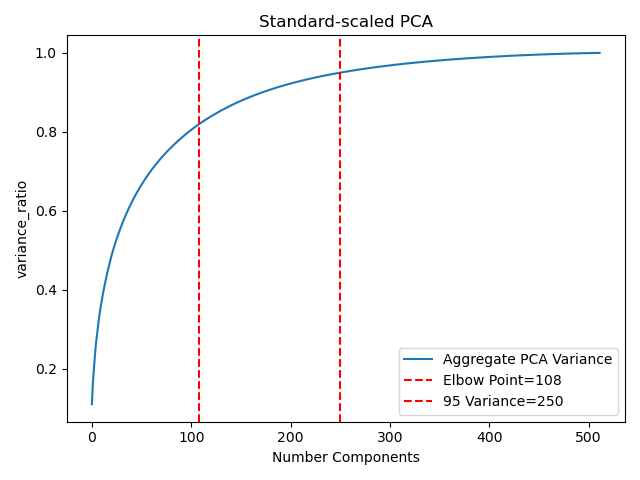
\includegraphics[width=.95\textwidth]{../../results_Experiment1/Standard_PCA_choice.png}
        \caption{Standard Scaler PCA Variance}
      \end{subfigure}
      \caption{Initial PCA choice experiment}
      \label{figure1}
\end{figure}

\section{Experiment 1}
For my first experiment, I used only 1/4 of the data, and quite a large grid search of sparse options for most 
items.  My goal was to discover which scaler worked best, and prod to see what behavior a PCA analysis invokes. 
Looking at the plots for the PCA variance in \ref{figure1}, I discovered that the elbow point was located close 
to the 80\% variance mark, and that the 95\% variance mark would still result in a respectable amount of dimensionality
reduction. As such, I locked my PCA search to be between .80 and .96 for all items. I did only use the accuracy metric 
for these first few experiments since my pre-existing codebase was hardcoded to use only the accuracy metric, and attempting
to fix it constituted a larger endeavor than I felt necessary for initial experiments.

\subsection{MLPNet}
\begin{figure}
    \begin{subfigure}{.5\textwidth}
        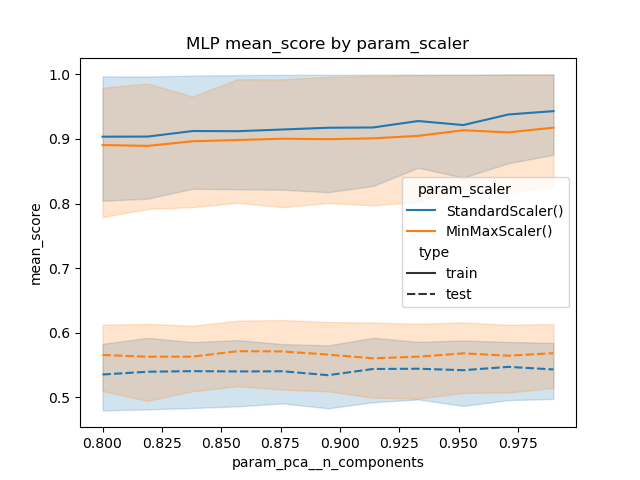
\includegraphics[width=.95\textwidth]{../../results_Experiment1/mlp/param_scaler_mean_score_param_pca__n_components.png}
        \caption{Scaler Choice By PCA}
        \end{subfigure}%
      \begin{subfigure}{.5\textwidth}
        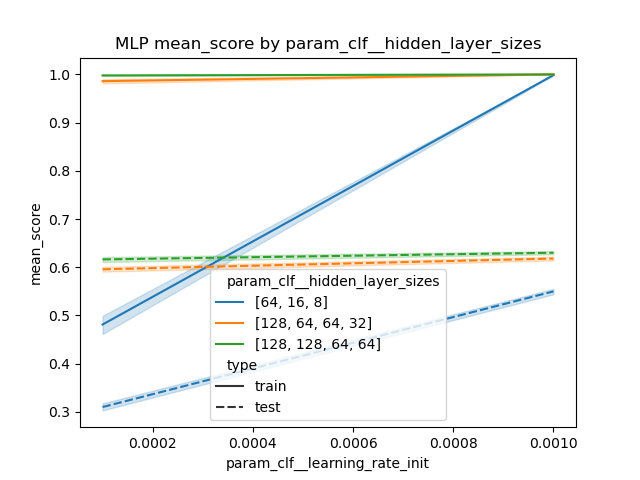
\includegraphics[width=.95\textwidth]{../../results_Experiment1/mlp/param_clf__hidden_layer_sizes_mean_score_param_clf__learning_rate_init.png}
        \caption{Model Choice by Learning Rate}
      \end{subfigure}
      \caption{MLPNet Experiment 1}
      \label{figure2}
\end{figure}

I had 3 major conclusions for the MLPNet which can be shown by these two plots in \ref{figure2}. First, We can see 
that across the board the minmax scaler appeard to be the correct choice of scaling. Across all metric combinations,
the minmax scaler both showed higher validation accuracy, and less over fitting than the standard scaler. So, 
I locked in the minmax scaler for all future experiments for the MLPNet classifier.

Second, we can see very minimal increase in performance across the PCA search, but we do see some slight improvements 
once we reach into the 90\% variance range. To check this, in the next experiment I cut down my search to be in the 90s
with the same amount of points, leading to a tighter search.

Finally, the more advanced network appeared to vastly out perform the simpler one. So, I increased model complexity for 
subsequent experiments.

\subsection{GNB}
The GNB results were the most straightforward. Oddly enough, the MinMax scaler appeared to perform the best, even though 
one would think a Gaussian-based preprocessing technique would be the best for a Gaussian-based classifier.

Due to the speed of this classifier, and the lack of other hyperparameters to tune, I was able to more densly pack the 
PCA search for this one. This led to an interesting discovery. For some reason, the scaling options all meet in 
validation performance at one point, before the minmax scaler proves to be the best for a short while, then the 
passthrough takes over again as performance degrades at the highest end of pca variance.

One thing I found interesting, was that this classifier did not show the usual improvements in fit time when the dimensionality
was lower. In fact, they saw remarkable improvements to fit times as the PCA approached maximum dimensionality.

Regardless, the GNB is serving it's purpose for me. I can see that the baseline accuracy should be greater than about .6,
and I can see that the linear separability of classes does indeed improve if given even the slightest amount of dimensionality
reduction. 

\begin{figure}
    \begin{subfigure}{.5\textwidth}
        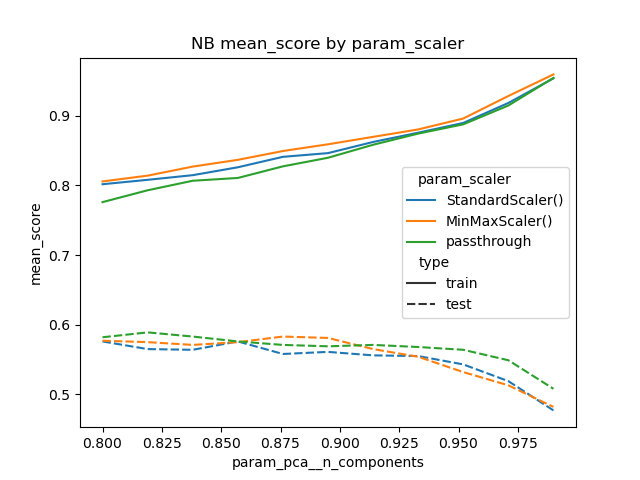
\includegraphics[width=.95\textwidth]{../../results_Experiment1/nb/param_scaler_mean_score_param_pca__n_components.png}
        \caption{Scaler Choice By PCA score}
        \end{subfigure}%
      \begin{subfigure}{.5\textwidth}
        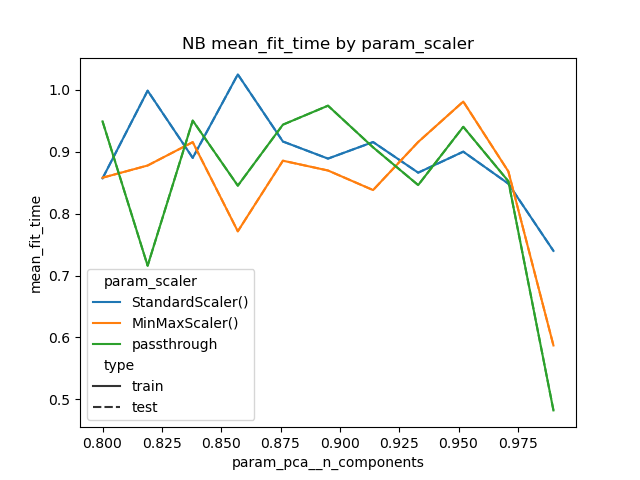
\includegraphics[width=.95\textwidth]{../../results_Experiment1/nb/param_scaler_mean_fit_time_param_pca__n_components.png}
        \caption{Scaler Choice by PCA Train Time}
      \end{subfigure}
      \caption{GNB Experiment 1}
      \label{figure3}
\end{figure}

\subsection{RF}

For the remaining classifiers, I will more quickly sum up the observations and conclusions as the broader information has 
already been covered.

For the RF classifier, we see nearly identical performance drop off at high levels of PCA variance that we saw in the 
GNB classifier, which is good for us because that means we can cut down the PCA to be in the 80s with respect to variance.

We can also see that the classifier behaves the best when we use no normalization, and that the sqrt method of feature 
selection appears to outpace the log2 method.

It appears that we could use more estimators likely, but I was planning on reserving that and the maximum depth searches 
for the next iteration of experiments.

\begin{figure}
    \begin{subfigure}{.5\textwidth}
        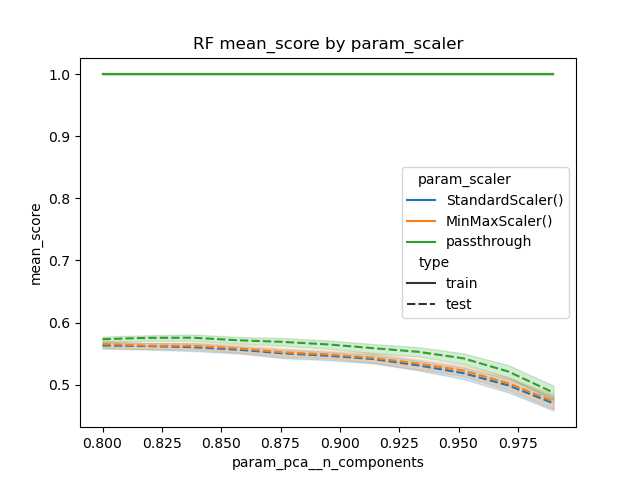
\includegraphics[width=.95\textwidth]{../../results_Experiment1/rf/param_scaler_mean_score_param_pca__n_components.png}
        \caption{Scaler Choice By PCA score}
        \end{subfigure}%
      \begin{subfigure}{.5\textwidth}
        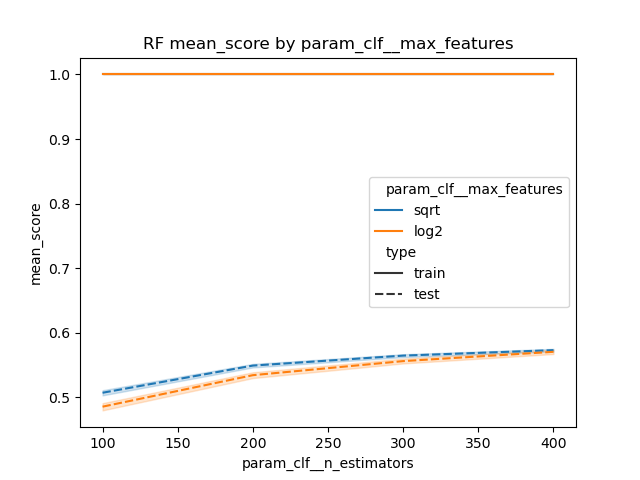
\includegraphics[width=.95\textwidth]{../../results_Experiment1/rf/param_clf__max_features_mean_score_param_clf__n_estimators.png}
        \caption{Feature choice by N Estimators}
      \end{subfigure}
      \caption{RF Experiment 1}
      \label{figure4}
\end{figure}

\subsection{SVM}

For our last model, the SVM, I decided to only test for rbf and sigmoid kernels to save time, and it appears that nothing 
is working at all for this classifier. We are getting moderately better results with the MinMax scaler, but they 
are still hanging around the .2 accuracy mark. 

We are seeing that lower PCA values are moderately better, but that's likely due to the fact that this experiment used 
only 1/4 of the data.

I can't make any strong conclusions for the SVM yet, but I will lock in the MinMax scaler as the best option, while 
also lowering Gamma since it appears like lower was better.

\begin{figure}
    \begin{subfigure}{.5\textwidth}
        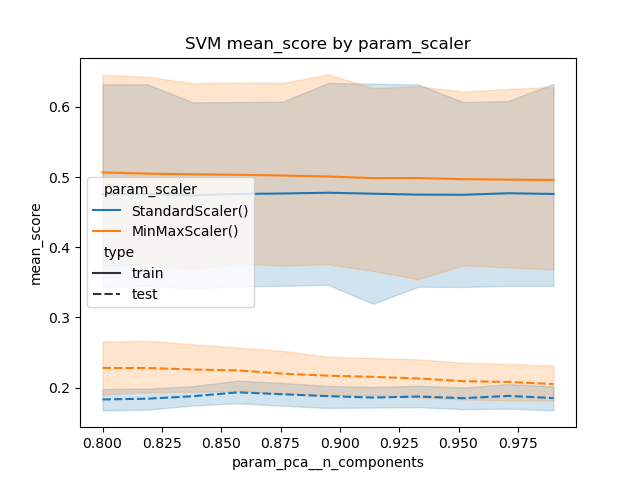
\includegraphics[width=.95\textwidth]{../../results_Experiment1/svm/param_scaler_mean_score_param_pca__n_components.png}
        \caption{Scaler Choice By PCA score}
        \end{subfigure}%
      \begin{subfigure}{.5\textwidth}
        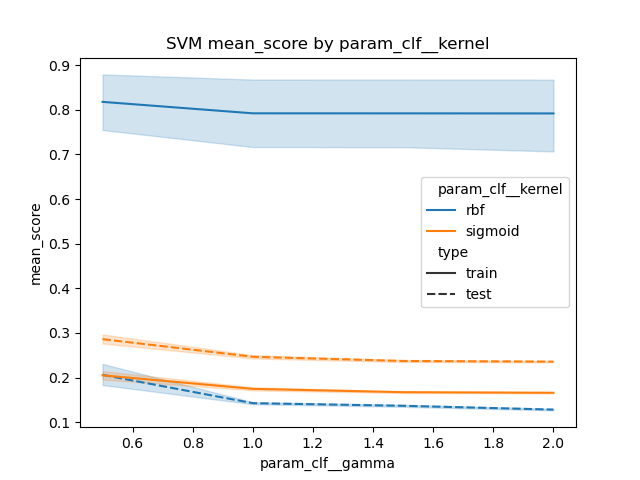
\includegraphics[width=.95\textwidth]{../../results_Experiment1/svm/param_clf__kernel_mean_score_param_clf__gamma.png}
        \caption{Kernel choice by Gamma}
      \end{subfigure}
      \caption{SVM Experiment 1}
      \label{figure5}
\end{figure}

\section{Experiment 2}
For this experiment, I'm still sticking with only looking at accuracy, but my goal is to tighten my searches a bit and 
confirm I'm moving in the right direction from Experiment 1. I'm moving on to use half of the data for this instead of 1/4
of the data.

I will more succinctly discuss the results and conclusions for this experiment since much of the justification for my choices 
will stay the same.

\subsection{MLPNet}
\begin{figure}
    \begin{subfigure}{.5\textwidth}
        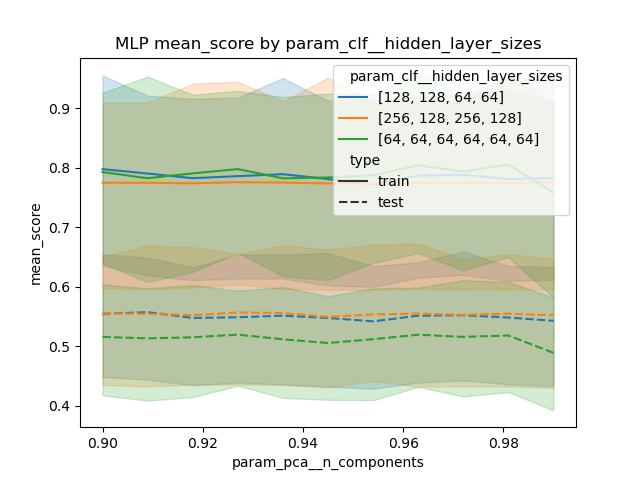
\includegraphics[width=.95\textwidth]{../../results_Experiment2/mlp/param_clf__hidden_layer_sizes_mean_score_param_pca__n_components.png}
        \caption{Effect of PCA on Performance}
        \end{subfigure}%
      \begin{subfigure}{.5\textwidth}
        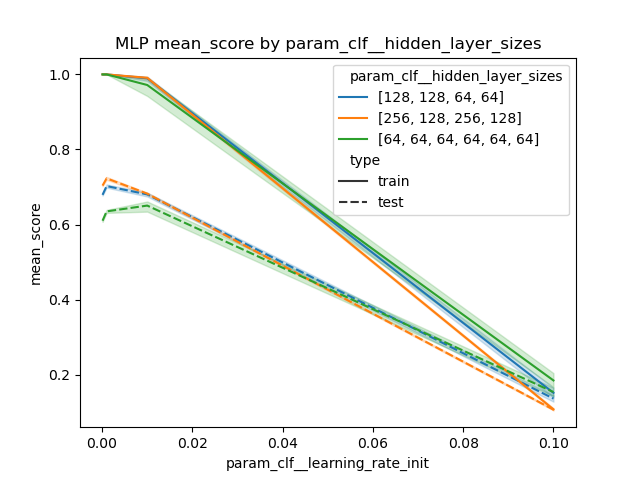
\includegraphics[width=.95\textwidth]{../../results_Experiment2/mlp/param_clf__hidden_layer_sizes_mean_score_param_clf__learning_rate_init.png}
        \caption{Effect of Learning Rate on Performance}
      \end{subfigure}
      \caption{MLPNet Experiment 2}
      \label{figure6}
\end{figure}

We can see that PCA had little influence on the performance of the models across, regardless of model complexity. 
As such, I'm likely going to keep it on the higher side for now since we will be adding more data as we progress, and 
the trend appears to be that more complex models work better.

Learning rate was the highest driver of performance, with a nearly linear relationship between performance and value, 
and very little variance denoted by the lightly colored region. Thus, low learning rate still wins out.

\subsection{GNB}
Results are almost identical to before, even with the increased data size. I'm expecting a large jump in performance 
once I use KMeans projections due to the centroid-based nature of the method.

\begin{figure}
    \begin{subfigure}{.5\textwidth}
        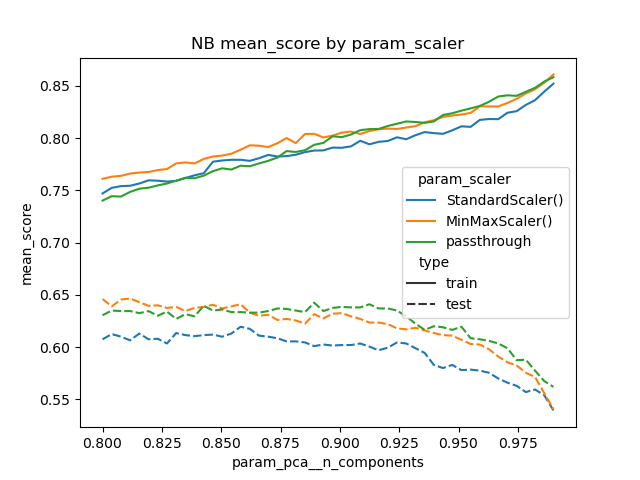
\includegraphics[width=.95\textwidth]{../../results_Experiment2/nb/param_scaler_mean_score_param_pca__n_components.png}
        \caption{Scaler Choice By PCA score}
        \end{subfigure}%
      \begin{subfigure}{.5\textwidth}
        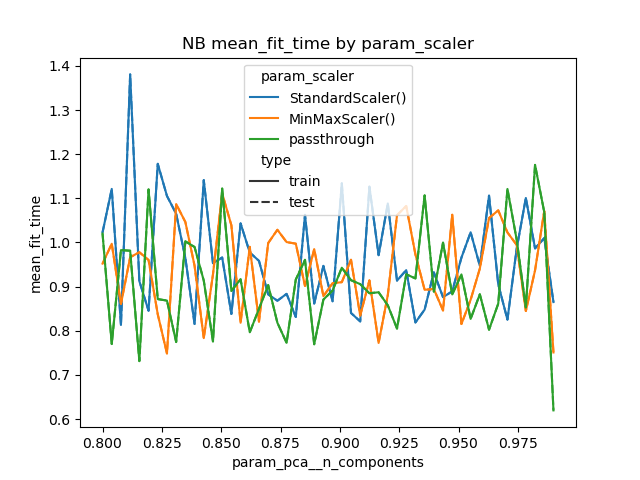
\includegraphics[width=.95\textwidth]{../../results_Experiment2/nb/param_scaler_mean_fit_time_param_pca__n_components.png}
        \caption{Scaler Choice by PCA Train Time}
      \end{subfigure}
      \caption{GNB Experiment 2}
      \label{figure7}
\end{figure}

\subsection{RF}

Higher estimators are better, for sure. The changes I made seemed to have given improvement and no new surprises 
when we doubled the amount of data. For this experiment, since I'd locked in what scaler I'm using I decided to plot the 
PCA variance vs. the number of estimators as a heat map, particularly due to the density of the search.

This plot challenges my previous thought that lower PCA was better, since it appears like there's a general improvement 
just before 90\%. I will move my search window to be centered at 90\% in the future.

\begin{figure}
    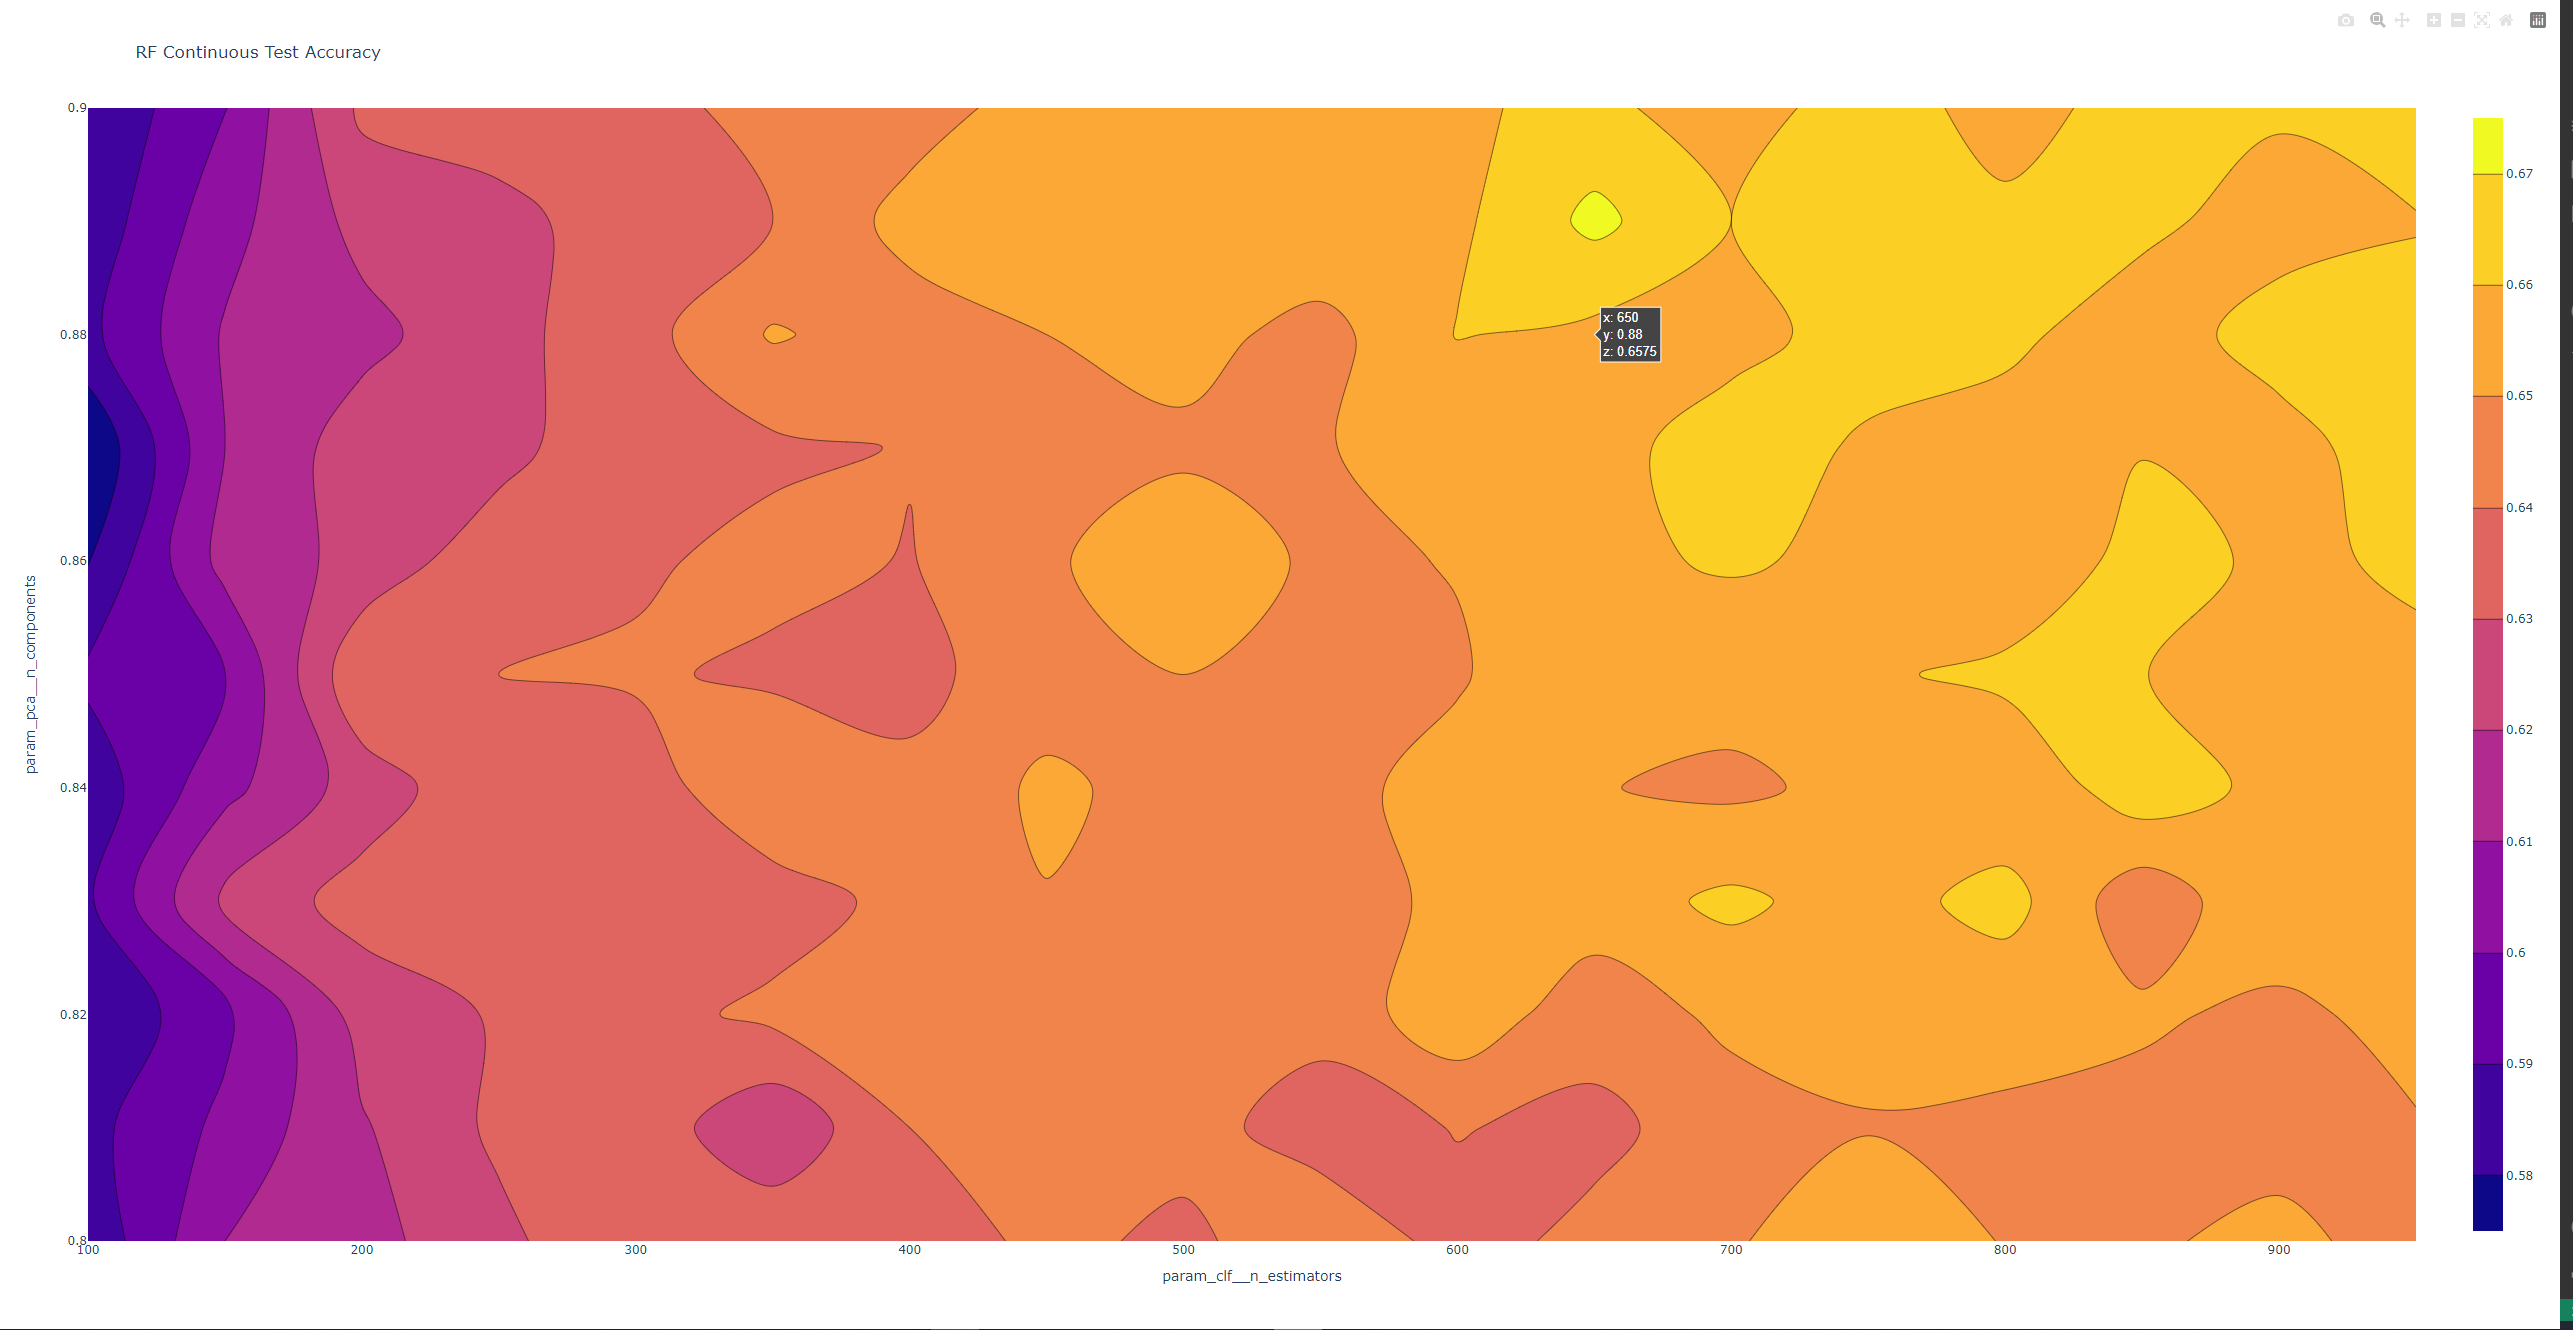
\includegraphics[width=.95\textwidth]{../../results_Experiment2/rf/Contour.PNG}
    \caption{Contour Plot of Variance vs. N Estimators}
    \label{figure8}
\end{figure}

\subsection{SVM}

\begin{figure}
    \begin{subfigure}{.5\textwidth}
        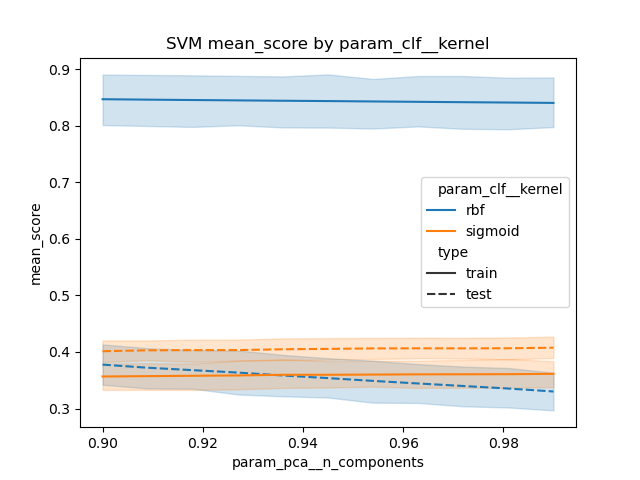
\includegraphics[width=.95\textwidth]{../../results_Experiment2/svm/param_clf__kernel_mean_score_param_pca__n_components.png}
        \caption{Kernel Choice By PCA score}
        \end{subfigure}%
      \begin{subfigure}{.5\textwidth}
        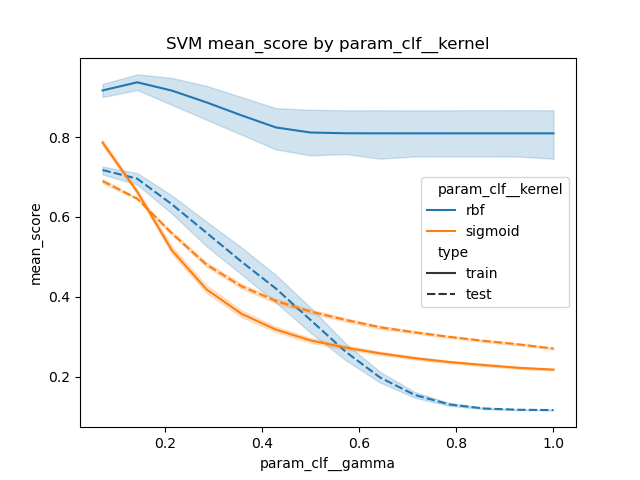
\includegraphics[width=.95\textwidth]{../../results_Experiment2/svm/param_clf__kernel_mean_score_param_clf__gamma.png}
        \caption{Kernel choice by Gamma}
      \end{subfigure}
    \begin{subfigure}{.95\textwidth}
        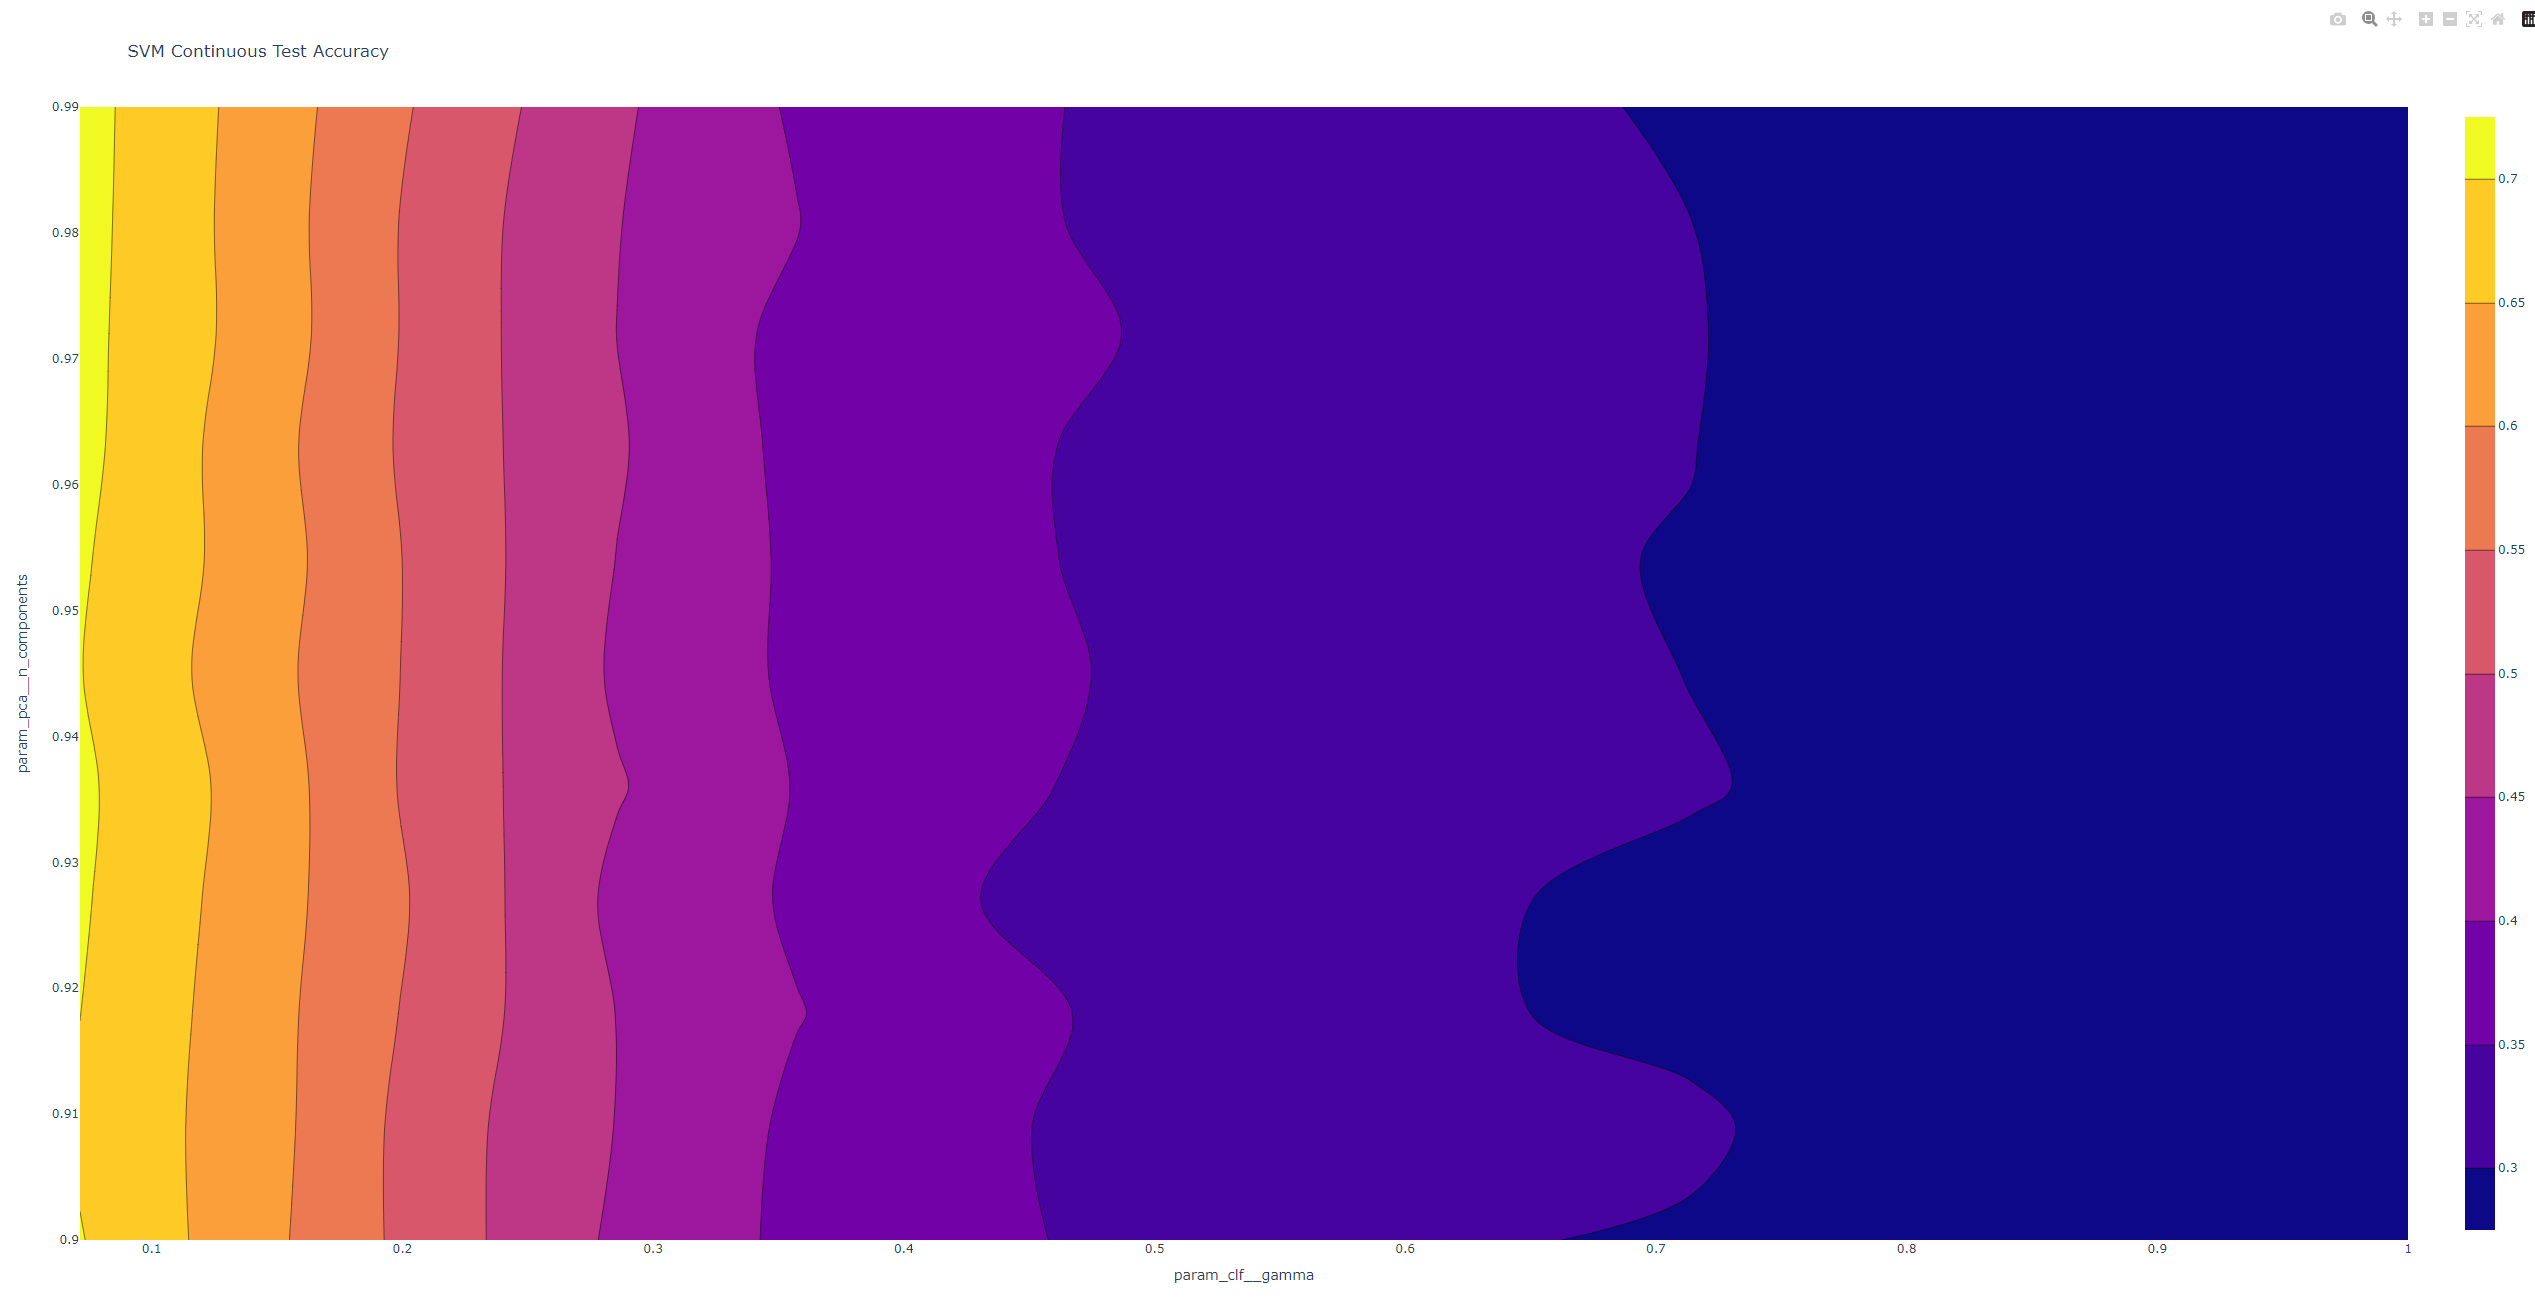
\includegraphics[width=.95\textwidth]{../../results_Experiment2/svm/Contour.PNG}
        \caption{Gamma vs. PCA Contour}
    \end{subfigure}
    \caption{SVM Experiment 2}
    \label{figure9}
\end{figure}

In this experiment, we can start to see the rbf kernel pull ahead of the sigmoid kernel in some areas, but not by enough 
to justify locking in our choice. We are going to have to stick with both of them for now, but I'm expecting the rbf kernel 
to start to pull ahead once we enter cluster transformations into the mix in the next steps.

Looking at the contour plot of PCA vs. gamma, I think it's pretty clear that low gamma and higher PCA variance appear to 
have the edge in the gridsearch. So, I'm going to keep PCA high, and gamma low.

\section{What Remains}
I've mostly expanded my analysis pipeline to include other forms of scoring. I do still have to work the kinks out of 
a couple of the more automated parts, but I expect to have that done long before you read this. This has been the biggest 
hurdle so far, but I expect to be over it soon.

For the cluster mapping requirement, I have decided to go a bit more hands-on for this. I ran KMeans clustering for a number 
of clusters ranging from 1 to 520, and calculated the gross cluster purity of the clusters. This basically means that 
for each cluster, I count how many of the samples are correctly grouped in a cluster where their class matches the majority 
of classes in that cluster. The result of this experiment is in \ref{figure10}.

\begin{figure}
    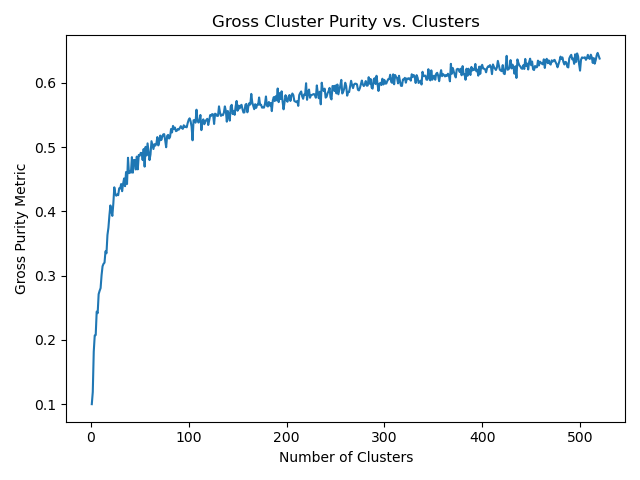
\includegraphics[width=.95\textwidth]{../../results/Cluster_Choice_Gross_Purity_larger.png}
    \caption{Cluster Analysis}
    \label{figure10}
\end{figure}

My goal for this is to use the clusters as dimensionality reduction, so that is why I am not going to go above 520 clusters.
As we can see in the plot, we quickly approach a an area where it begins to taper off around 60-100 clusters, and becomes
almost linear beyond that. However, since running the cluster analysis to generate these is quite time consuming (unlike PCA)
I plan on only using 2 different cluster transformations whcih are 100, and 200 clusters to meet the minimum requirement for 
the assignment. If I have time and see the benefit, I might do more.


I have not begun yet on the ensemble methods, but I plan to use the best performing item from each of the 4 different classifiers, and 
ensuring that at least 2 models use the kmeans transformations in order to ensure we have good variance of our classifiers.

\end{document}